\documentclass[a4paper]{article}

%% Language and font encodings
\usepackage[english]{babel}
\usepackage[utf8x]{inputenc}
\usepackage[T1]{fontenc}
\usepackage[table]{xcolor}

%% Sets page size and margins
\usepackage[a4paper,top=3cm,bottom=2cm,left=3cm,right=3cm,marginparwidth=1.75cm]{geometry}

%% Useful packages
\usepackage{amsmath}
\usepackage{graphicx}
\usepackage{subcaption}
\usepackage[colorinlistoftodos]{todonotes}
\usepackage[colorlinks=true, allcolors=blue]{hyperref}

\usepackage{multirow}


%\title{Investigating Blip Glitches Using GravitySpy and Q-Transforms to Find Sub-Classes}
\title{Sub-Classification of Blip Glitches Using Q-Transforms and Convolutional Neural Networks with GravitySpy}
\author{Melissa Kohl}
\date{\today}

\begin{document}
\maketitle
\graphicspath{ {images/} }

\begin{abstract}

In the Advanced LIGO observation runs, detection of gravitational waves is directly dependent on the sensitivity of the detectors. Transient noise, called "glitches," not only affects the general sensitivity of the detectors along with continuous noise, but also mimics and obscures real gravitational waves in the calibrated strain data channel. One machine learning software package used to classify these glitches and identify their sources, GravitySpy\footnote{\href{https://gravity-spy.github.io}{GravitySpy documentation}}, is successful when the spectrogram of the glitch has a very distinct and unique shape. However, GravitySpy's spectrogram of one of the most common types of glitches, called a "blip," has an indistinct shape due to so few cycles being in-band, and tends to ring off template signals of binary black hole mergers, making it especially necessary to eliminate blips for future observing runs. Additionally, auxiliary channels other than the calibrated strain can pick up glitches and supplement GravitySpy's search for sources, but blip glitches are very infrequently witnessed by other channels and therefore still have unknown sources. The focus of this paper is to examine blip glitches in a Q-transform spectrogram with different parameters than those used by GravitySpy to determine if there are sub-classifications of blips that might have identifiable sources, and then use Convolutional Neural Networks to sub-classify these blips. Manual searches of short-duration Q-transform spectrograms of random blip glitches, nearly indistinguishable in GravitySpy's spectrograms, reveal six distinct possible subclasses. In addition, the implementation of Convolutional Neural Networks has provided preliminary evidence of fundamental differences between these hypothesized subclasses, confirming the assumption that there are multiple types of blips and aiding in future searches for blip sources.

\end{abstract} 

\section{Introduction to Glitch Classification} \label{introduction}

The glitches in the strain data from the science and observation runs of the Advanced LIGO detectors decrease the sensitivity of the detectors and obscure gravitational waves \cite{Zevin:2016}. Although some glitches can be identified and eliminated from the strain data during later analysis, astronomical events that give off additional radiation, such as neutron star mergers, need to be recognized immediately so that astronomers can observe the event. Additionally, the shapes of some glitches, such as "blip" glitches, mimic that of a gravitational wave from a binary black hole merger so well that one of the only ways to distinguish a blip from a gravitational wave is by comparing the data between detectors. As a result, it is imperative to find the sources of the glitches and eliminate them before future observing runs, directly increasing the sensitivity and effectiveness of the detectors while observing \cite{Mukherjee:2010}. 

The current method for classifying glitches and identifying their sources is a machine learning software package called GravitySpy \cite{Zevin:2016}. Unlike previous machine learning techniques used on LIGO data that only looked at the waveforms of the glitches \cite{Mukherjee:2010}, GravitySpy's neural network takes in spectrograms from four different time frames to create a multi-input network that utilizes image classification techniques \cite{Bahaadini:2017}. Since different types of glitches have different durations, the multiple views not only provide complementary data across time frames, but also allow for identification of a broader group of glitches of different durations \cite{Bahaadini:2017}. GravitySpy also relies on citizen science to classify glitches, utilizing a large volunteer network to aid in adding glitches to the neural network training set\footnote{\href{https://www.zooniverse.org/projects/zooniverse/gravity-spy}{GravitySpy Zooniverse}}. As a result, GravitySpy is great at classifying glitches into known classifications \cite{Zevin:2016}, but the classifications themselves may be too broad. The output function in GravitySpy's neural network is \texttt{softmax} \cite{Bahaadini:2017}, which essentially just classifies the input glitch into the classification with the highest correlation, regardless of how high that correlation is. The combination of the multiple-view input and the \texttt{softmax} output function allow for glitches caused by different sources to be classified into the same group if the shapes of the glitches are similar. In section \ref{investigation}, I introduce an example of two different spectrogram shapes (which most likely have different sources) that are grouped into the same classification. 

Once glitches are classified, GravitySpy is also used to find similar glitches in the hundreds of thousands of auxiliary channels keeping track of the instruments and environments of each detector in an attempt to locate the source of each glitch classification \cite{Zevin:2016}. Currently, this method is insufficient for finding an identifiable source of blip glitches, largely due to a lack of channels witnessing blip glitches.

\section{Initial Approach and Goals} \label{goal}

The most frequently-occurring glitches, including blip glitches, are likely conglomerates of glitches from different sources that happen to create the same general shape in a spectrogram. Unfortunately, the shape of a blip glitch in GravitySpy's spectrogram is uninspiring, with no weird spikes or unique shapes to provide a hint towards its source, and little to even distinguish one from another. In comparison with other glitches, such as whistles, blips have an extremely short duration, which could contribute to the lack of visible characteristics. As mentioned in the previous section, blip glitches are also troublesome due to their resemblance to binary black hole mergers. To sub-classify these blip glitches for future elimination, we first need a different analysis technique that might reveal hidden characteristics. 

One common way to visualize a glitch or other transient noise waveform in the strain data is a Q-transform, which is a time-to-frequency domain transform related to the Fourier transform. The quality factor Q is related to the number of cycles processed at a central frequency, and in comparison with a Fourier transform, the Q-transform has a better frequency resolution over a logarithmic frequency scale, and a better resolution for short duration signals. Since the glitches (and blips in particular) and gravitational waves in the Advanced LIGO strain data have a very short duration and span auditory frequencies, which are on a logarithmic scale, the Q-transform is a more desirable time-to-frequency domain transform for our purposes than the Fourier transform. Additionally, while the Q-transform produces a spectrogram very similar to the spectrograms used by GravitySpy, the parameters set by GravitySpy are designed to help visualize the blip over larger time frames, and my goal is to use the Q-transform to zoom in on the blip glitches to see possible characteristics over a small time frame.

Once we find distinguishable subclasses of blip glitches in Q-transform images, we can use those images as input to different neural networks to build a neural network that can sort the blips into sub-classifications. If we can identify clusters and groupings of blips using different neural networks, there is a possibility of identifying the specific characteristics that define the subclasses. Without sub-classification, GravitySpy cannot identify the sources of blip glitches, but with a new input set, the possibility of finding a source and reducing some of the transient noise caused by blip glitches is largely increased. 

\section{Investigation of Blip Glitches}

\subsection{Initial Look at O1 Blips from Livingston} \label{investigation}

To gain a better understanding of blip glitches and their characteristics, I started by performing simple Q-transforms on known blip glitches from the first observing run at the Livingston detector. I wrote a Python script, adapted from the GWpy\footnote{\href{https://gwpy.github.io/docs/stable/overview.html}{GWpy overview}} Q-transform documentation\footnote{\href{https://gwpy.github.io/docs/stable/examples/timeseries/qscan.html}{Q-Transform code example}}, to plot the Q-transform of about 30 random blip glitches, all cropped from the surrounding 30 seconds of strain data to a final image with a time domain of 0.30 seconds, with all other parameters held constant. While manually looking through the images, I found four distinct types of blip glitches, as seen in figure \ref{fig:q_transforms} on page \pageref{fig:q_transforms}. I call these four types normal, spread, dot, and stick for their appearances in the Q-transform. Since the shapes of these images are drastically different from each other, I made the assumption that at least one of these could be a subclass of blips.

\begin{figure}[h!]
	\centering
	\begin{subfigure}{.49\textwidth}
		\centering
		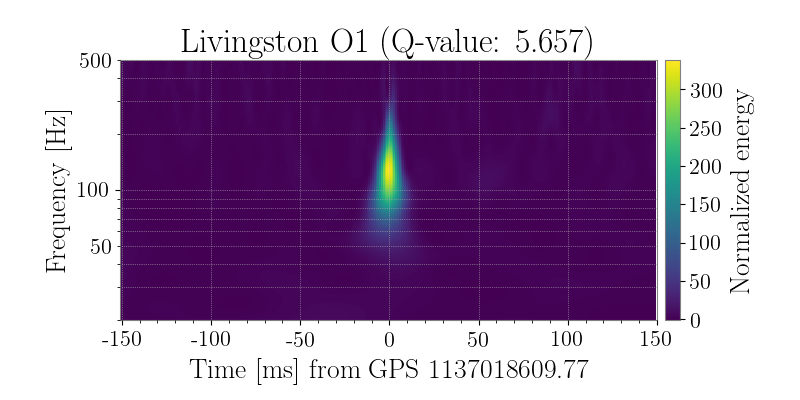
\includegraphics[width=1\linewidth]{normal_blip}
		\caption{Normal blip Q-transform}
		\label{fig:normal}
	\end{subfigure}
	\begin{subfigure}{.49\textwidth}
		\centering
		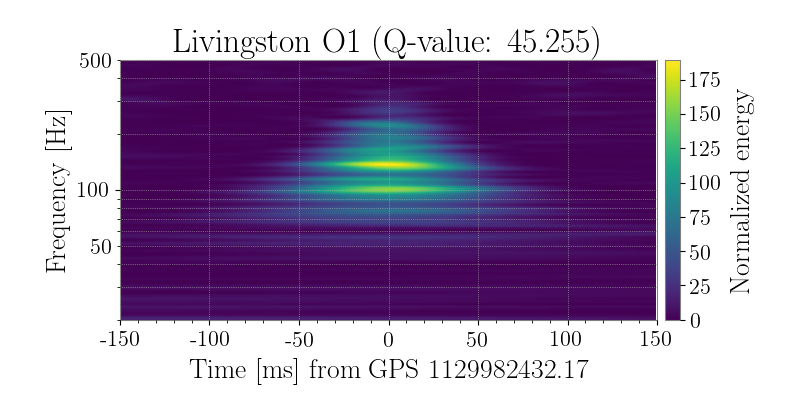
\includegraphics[width=1\linewidth]{spread_blip}
		\caption{Spread blip Q-transform}
		\label{fig:spread}
	\end{subfigure}
	\begin{subfigure}{.49\textwidth}
		\centering
		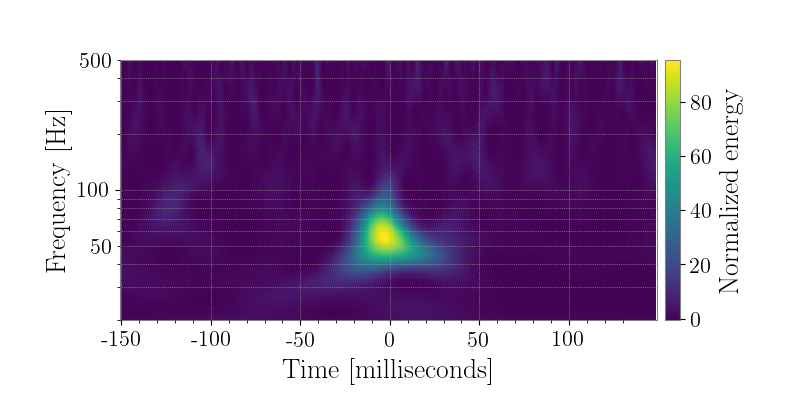
\includegraphics[width=1\linewidth]{dot_blip}
		\caption{Dot blip Q-transform}
		\label{fig:dot}
	\end{subfigure}
	\begin{subfigure}{.49\textwidth}
		\centering
		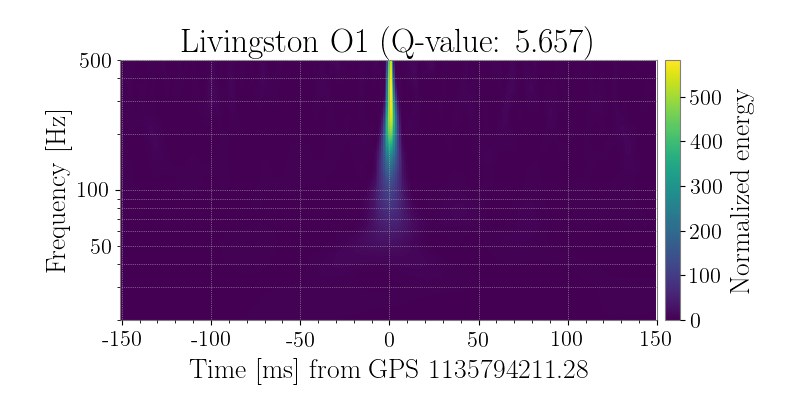
\includegraphics[width=1\linewidth]{stick_blip}
		\caption{Stick blip Q-transform}
		\label{fig:stick}
	\end{subfigure}
	\caption{Four different types of blip glitches from Livingston O1 in Q-transforms, all with the same time duration of 0.30 seconds, cropped from 30 seconds of transformed strain data. The Q-value calculated by GWpy is 5.65 for all but the spread blip (45.25). Note that the energy scale is different for each blip.}
	\label{fig:q_transforms}
\end{figure}

After discovering these differing forms in the Q-transforms, and plotting about 100 more Q-transforms, I looked at the existing GravitySpy spectrograms from LigoDV-Web of a specific blip from each of the four possible subclassifications to determine the legitimacy of my assumptions, the results of which are in figure \ref{fig:comparison} on page \pageref{fig:comparison}. (Note: Any future mention of a "spectrogram" refers to GravitySpy's spectrograms, and any future mention of a "Q-transform" refers to my own short-duration spectrograms.)

\begin{figure}[h!]
	\centering
	\begin{subfigure}[t]{.7\textwidth}
		\centering
		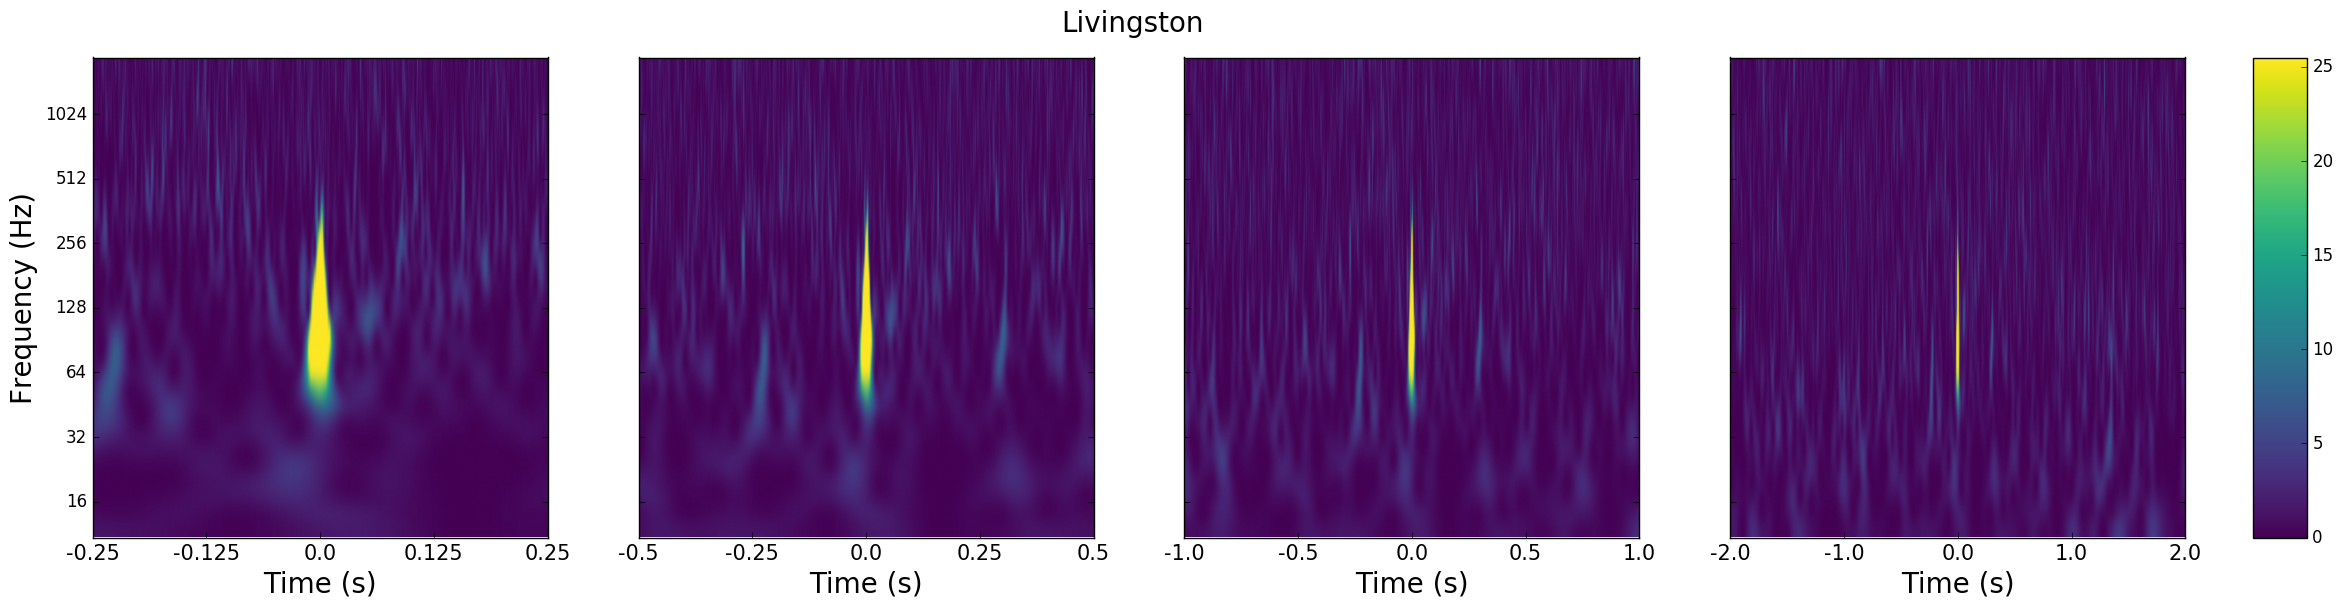
\includegraphics[width=.9\linewidth]{normal_blip_spect}
		\caption{Normal blip spectrograms}
		\label{fig:normal_s}
	\end{subfigure}
	\begin{subfigure}[t]{.29\textwidth}
		\centering
		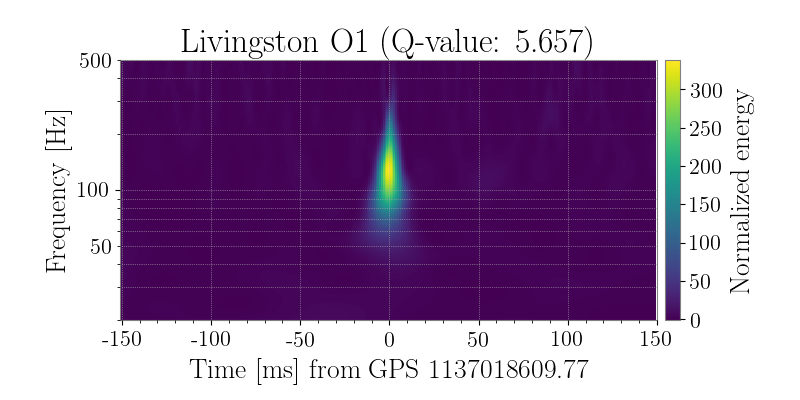
\includegraphics[width=1.1\linewidth]{normal_blip}
		\caption{Normal blip Q-transform}
		\label{fig:normal_q}
	\end{subfigure}
	\begin{subfigure}[t]{.7\textwidth}
		\centering
		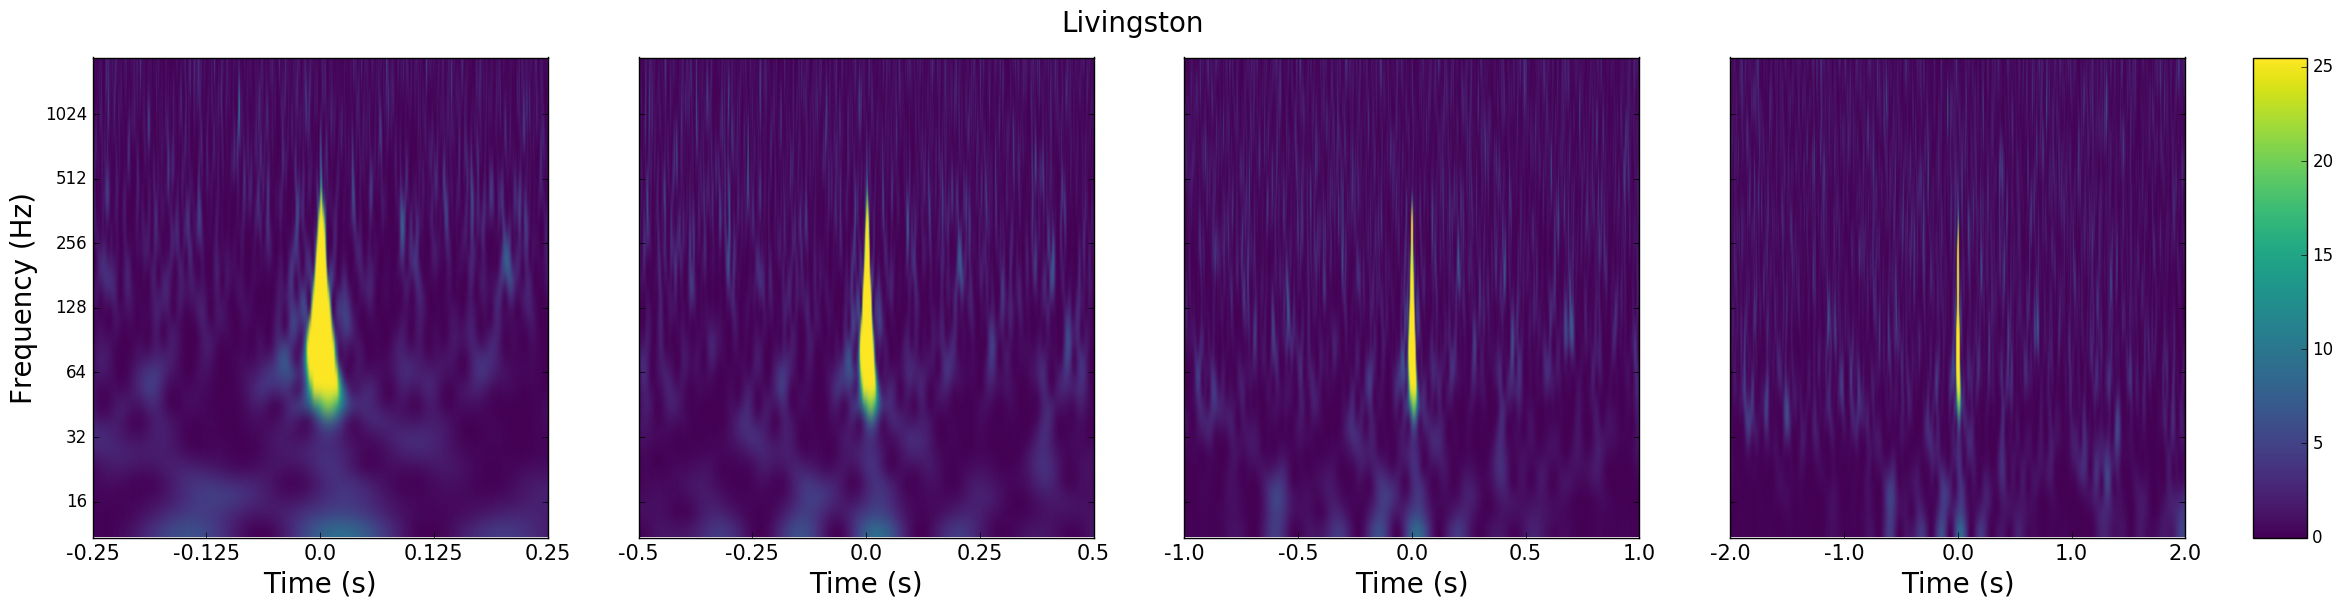
\includegraphics[width=.9\linewidth]{spread_blip_spect}
		\caption{Spread blip spectrograms}
		\label{fig:spread_s}
	\end{subfigure}
	\begin{subfigure}[t]{.29\textwidth}
		\centering
		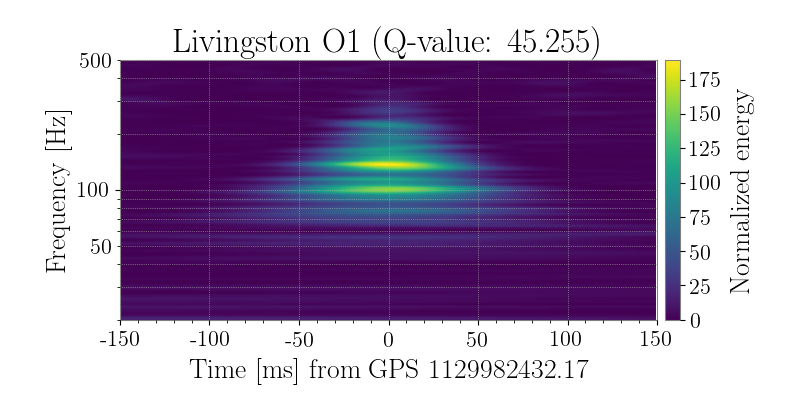
\includegraphics[width=1.1\linewidth]{spread_blip}
		\caption{Spread blip Q-transform}
		\label{fig:spread_q}
	\end{subfigure}
	\begin{subfigure}[t]{.7\textwidth}
		\centering
		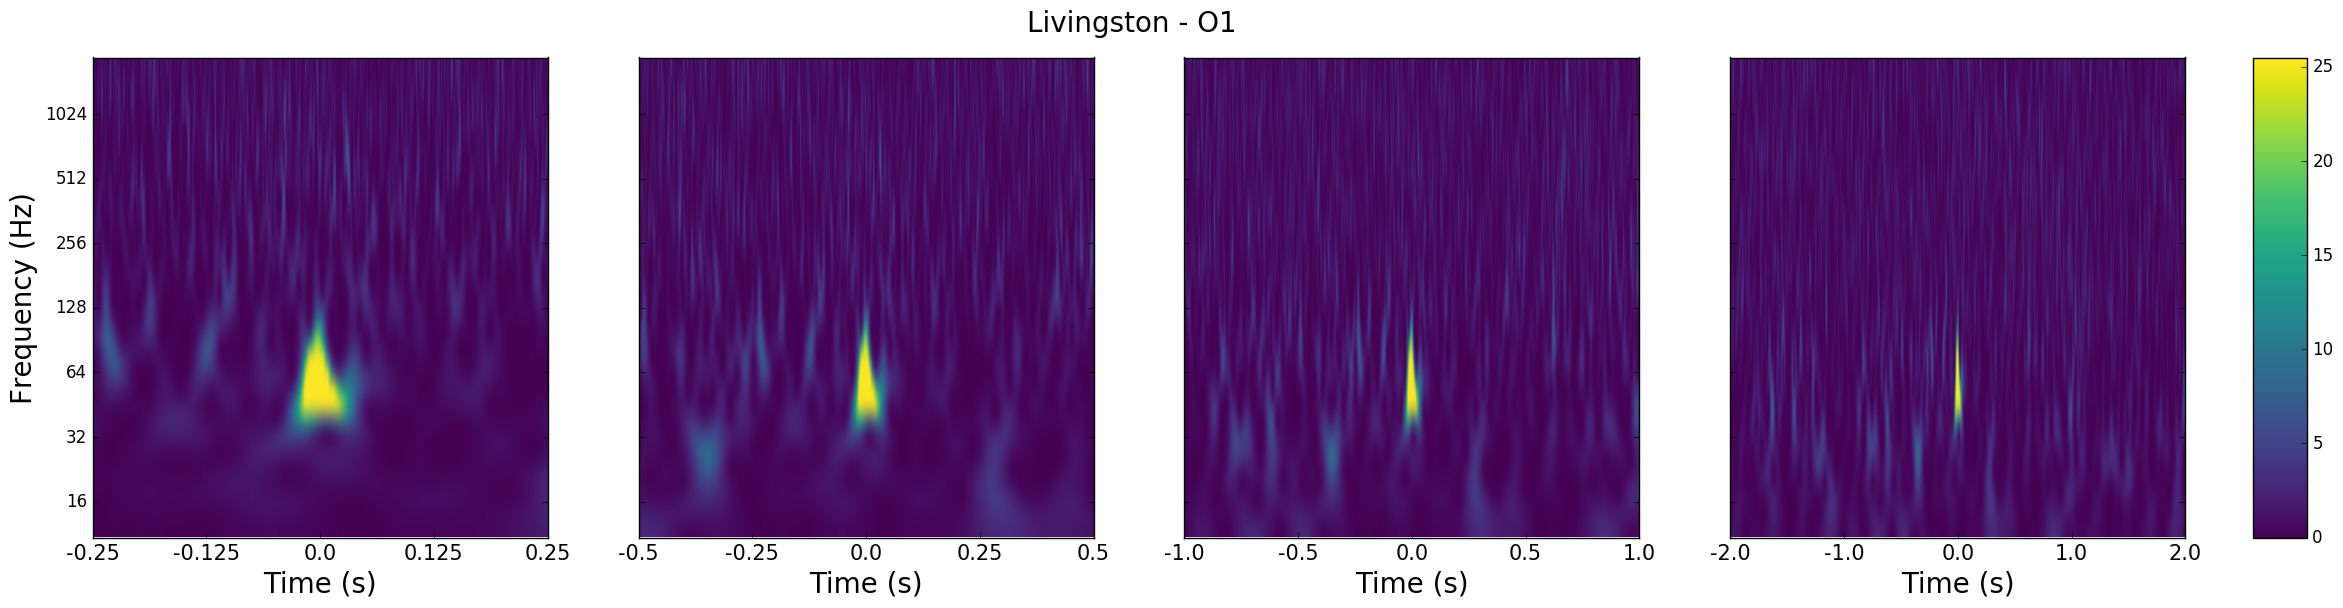
\includegraphics[width=.9\linewidth]{dot_blip_spect}
		\caption{Dot blip spectrograms}
		\label{fig:dot_s}
	\end{subfigure}
	\begin{subfigure}[t]{.29\textwidth}
		\centering
		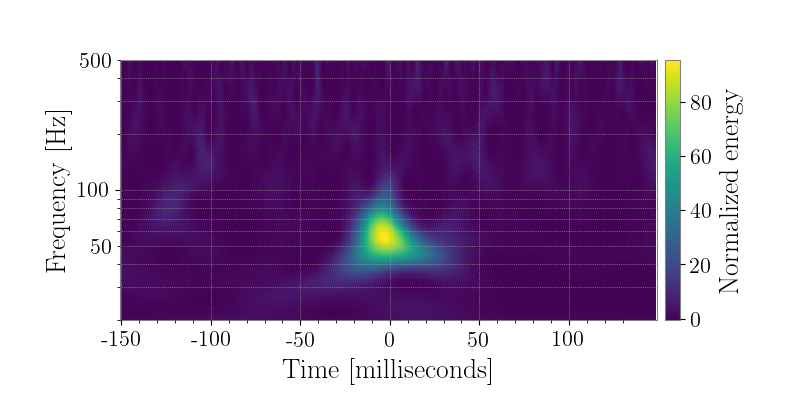
\includegraphics[width=1.1\linewidth]{dot_blip}
		\caption{Dot blip Q-transform}
		\label{fig:dot_q}
	\end{subfigure}
	\begin{subfigure}[t]{.7\textwidth}
		\centering
		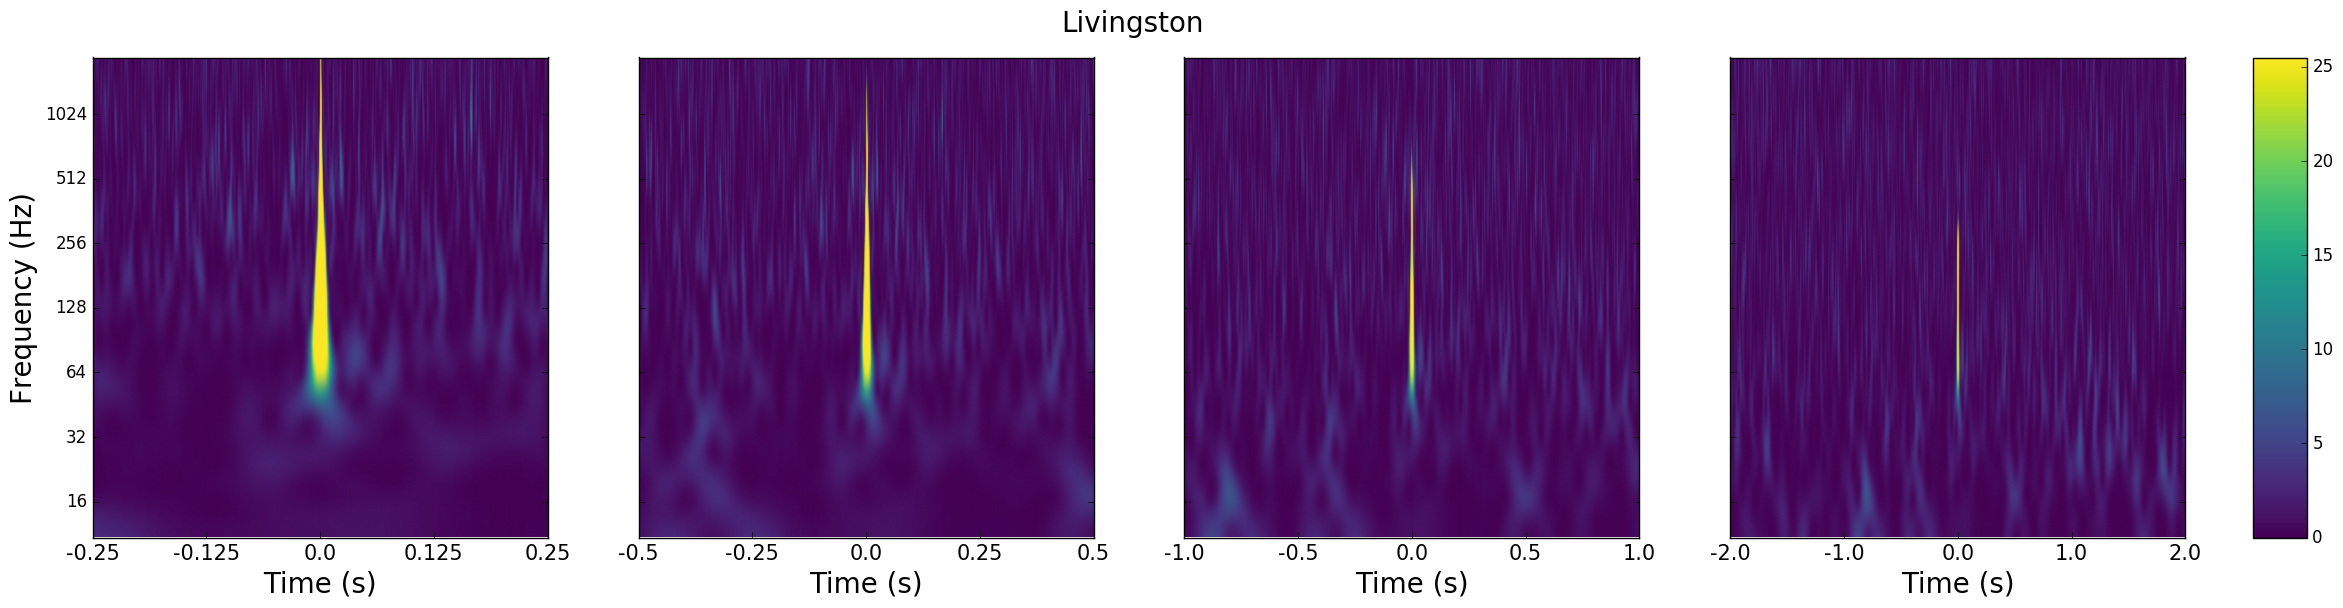
\includegraphics[width=.9\linewidth]{stick_blip_spect}
		\caption{Stick blip spectrograms}
		\label{fig:stick_s}
	\end{subfigure}
	\begin{subfigure}[t]{.29\textwidth}
		\centering
		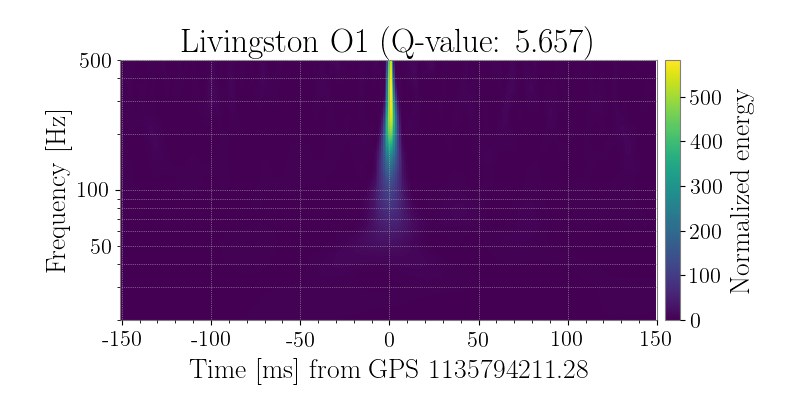
\includegraphics[width=1.1\linewidth]{stick_blip}
		\caption{Stick blip Q-transform}
		\label{fig:stick_q}
	\end{subfigure}
	\caption{A comparison between GravitySpy spectrograms of four different blip glitches on the left and the corresponding short-duration Q-transform of the same blip glitches on the right. The spectrogram images come from LigoDV-Web, with time durations from left to right of 0.5 seconds, 1.0 seconds, 2.0 seconds, and 4.0 seconds. The Q-transform images were created from my Python script, cropped from 30 seconds of transformed data down to 0.30 seconds. The top row is a normal blip, the second row is a spread blip, the third a dot blip, and a stick blip on the bottom. Although the spectrograms of the different blips are somewhat distinguishable from one another, the Q-transforms reveal that these blip glitches may have fundamental differences.}
	\label{fig:comparison}
\end{figure}

The most striking difference between the spectrograms and the Q-transforms is from the spread blip. The spectrograms from the normal blip and the spread blip, figures \ref{fig:normal_s} and \ref{fig:spread_s}, appear to be almost exactly the same, but while the normal blip's Q-transform (figure \ref{fig:normal_q}) has the same shape as its spectrogram, hence the name "normal," the spread blip's Q-transform (figure \ref{fig:spread_s}) "spreads" outward with distinct horizontal lines. These horizontal lines (which are essentially frequency bins) suggest that the duration of a spread blip is longer than the rest of the blips and therefore it needs more data than 30 seconds for a clear Q-transform. Additionally, the much larger Q-value (45.25) immediately suggests that something odd is going on with the transform.

The dot blip has a chance of being a legitimate sub-classification, as its Q-transform (figure \ref{fig:dot_q}) has a distinct round shape at a relatively low frequency compared to the other blips. Unlike the spread blip, however, the spectrogram of the dot blip (figure \ref{fig:dot_s}) is easily distinguishable from the others, with a much smaller frequency range and an almost triangle-like shape. This is an example of a possible distinguishable classification of glitch that GravitySpy groups in with blips, as mentioned in section \ref{introduction}. So, since a dot blip can be identified on a spectrogram, it is possible that it could be classified apart from other blip glitches by GravitySpy, but it is worth investigating possible attributes of dot blips, such as lower frequency and longer duration compared to other blips.

The stick blip also seems to be different than a normal blip. Its spectrogram (figure \ref{fig:stick_s}) is only slightly skinnier than that of a normal blip, with a slightly longer tail. However, the Q-transform (figure \ref{fig:stick_q}) reveals that a stick blip is at a significantly higher frequency than a normal blip. Even if the stick blip is the same shape as a normal blip, the higher frequency sets it apart, especially compared to dot blips.

In addition, this comparison between GravitySpy's spectrograms and my own Q-transforms validates GravitySpy's ability to classify similar images. The four shapes I found in the Q-transforms do not appear to be mis-classified, they simply have characteristics that cannot be discerned from GravitySpy's specific type of spectrogram.

\subsection{Further Investigation into O2 and Hanford Blips} \label{O2}

Before delving into possible characteristics that could separate the types of blips I had found, I wanted to clear up the spread blip's Q-transform and see whether the same variety of shapes from my findings in O1 at Livingston are present in O2 and/or at Hanford.

I attempted to condense the spread blips by creating another two Q-transforms for each spread blip using the surrounding 40 seconds and 60 seconds of data, rather than my original 30 seconds, thinking that the image wasn't clear due to the signal having a longer duration compared to other blips. However, the exact same spread effect occurred for all of the known spread blips for both widened time domains. So, I went the other direction and used the surrounding 20 seconds, which could indicate a problem with the internal whitening that occurs to create the spectrogram of the transform, rather than a signal duration problem. Fortunately, this shortening of the domain cleared the images and we could see the actual shapes of the spread blips, one example of which is in figure \ref{fig:spread_ex} on page \pageref{fig:spread_ex}.

\begin{figure}[h!]
	\centering
	\begin{subfigure}{.49\textwidth}
		\centering
		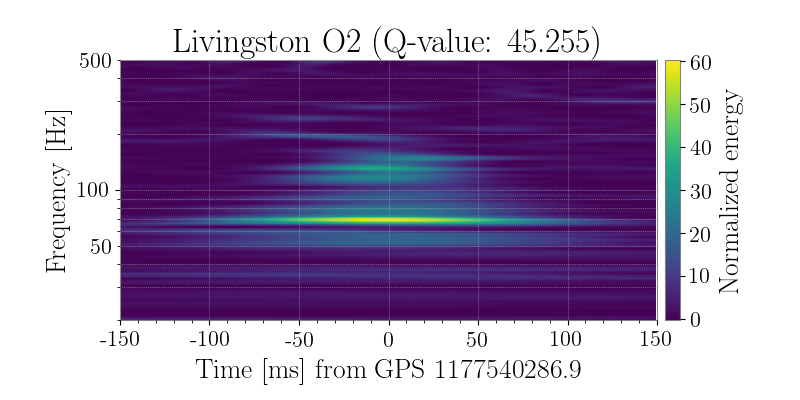
\includegraphics[width=1\linewidth]{spread_ex_30s}
		\caption{Spread blip with 30 second domain}
		\label{fig:spread_30}
	\end{subfigure}
	\begin{subfigure}{.49\textwidth}
		\centering
		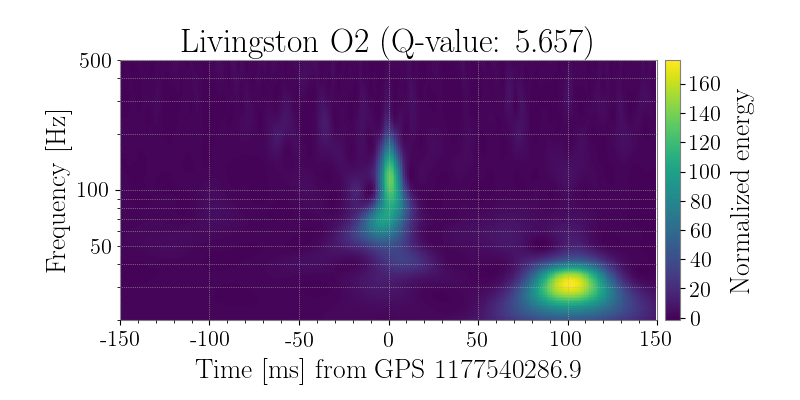
\includegraphics[width=1\linewidth]{spread_ex_20s}
		\caption{Spread blip with 20 second domain}
		\label{fig:spread_20}
	\end{subfigure}
	\caption{A blip glitch from Livingston O2 with two different amounts of surrounding data, both cropped back down to 0.3 seconds.}% Using a smaller domain reveals a double-blip, where there are two distinct signals about 100 milliseconds apart.}
	\label{fig:spread_ex}
\end{figure}

If not for the suspiciously large Q-value in figure \ref{fig:spread_30}, it would appear that the original time domain parameter of the Q-transform was simply obscuring the image. Some of the spreads condensed down to dot blips, others normals and sticks. The spread blip from figures \ref{fig:q_transforms} and \ref{fig:comparison} turned out to be a normal blip, explaining why the spectrogram of the normal blip was so similar to that of the spread blip in that case. However, a few spreads did not fit into the three initial possible subclasses, including a couple that appear to contain two different signals within 100 milliseconds of each other, such as figure \ref{fig:spread_20}, which I call a double-blip. Although changing the amount of data to get rid of the spreading effect in my Q-transforms is good enough for the purposes of this project, the reason behind this spreading is unknown and could be a future point of investigation.

Now knowing that 20 seconds is a more consistent parameter for the Q-transform than 30 seconds, and also knowing that there was a large possibility for other types of blips beyond dots, normals, and sticks, I plotted and classified around 150 blip glitches from Hanford O2 and about 100 blip glitches from Livingston O2. I found six major shapes of blips, all of which are at both detectors, as shown in figure \ref{fig:six} on page \pageref{fig:six}. The dot, stick, and normal are still there, but I also found double-blips, snitches (named for the Golden Snitch from \textit{Harry Potter}), and hats (named for the Sorting Hat from \textit{Harry Potter}). 

\begin{figure}[h!]
	\centering
	\begin{subfigure}{.49\textwidth}
		\centering
		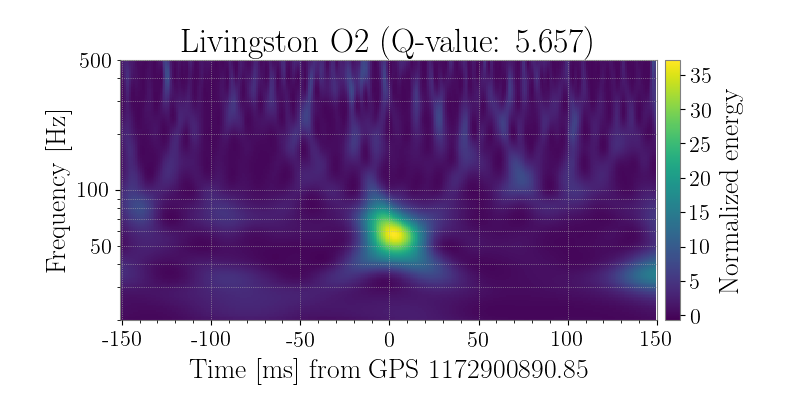
\includegraphics[width=1\linewidth]{dot_O2}
		\caption{Dot blip}
		\label{fig:dot_O2}
	\end{subfigure}
	\begin{subfigure}{.49\textwidth}
		\centering
		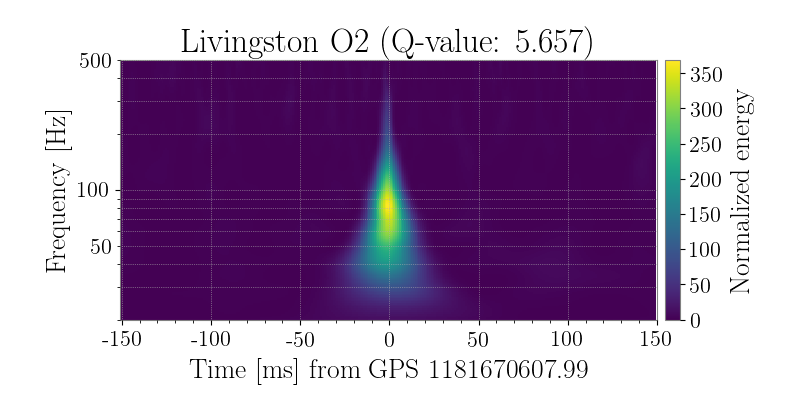
\includegraphics[width=1\linewidth]{normal_O2}
		\caption{Normal blip}
		\label{fig:normal_O2}
	\end{subfigure}
	\begin{subfigure}{.49\textwidth}
		\centering
		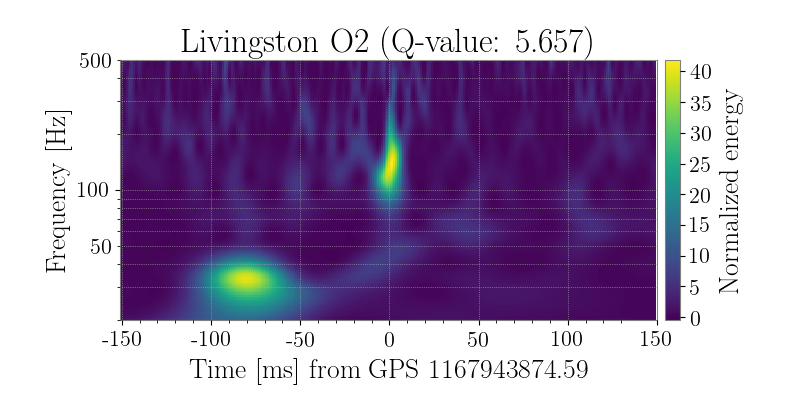
\includegraphics[width=1\linewidth]{double_O2}
		\caption{Double blip}
		\label{fig:double_O2}
	\end{subfigure}
	\begin{subfigure}{.49\textwidth}
		\centering
		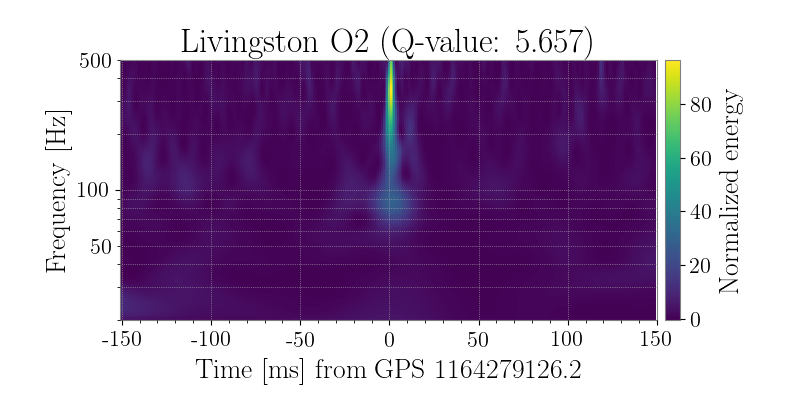
\includegraphics[width=1\linewidth]{stick_O2}
		\caption{Stick blip}
		\label{fig:stick_O2}
	\end{subfigure}
	\begin{subfigure}{.49\textwidth}
		\centering
		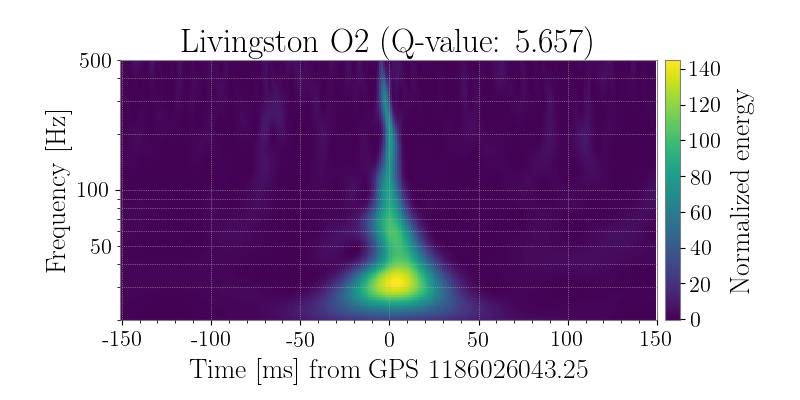
\includegraphics[width=1\linewidth]{hat_O2}
		\caption{Hat blip}
		\label{fig:hat_O2}
	\end{subfigure}
	\begin{subfigure}{.49\textwidth}
		\centering
		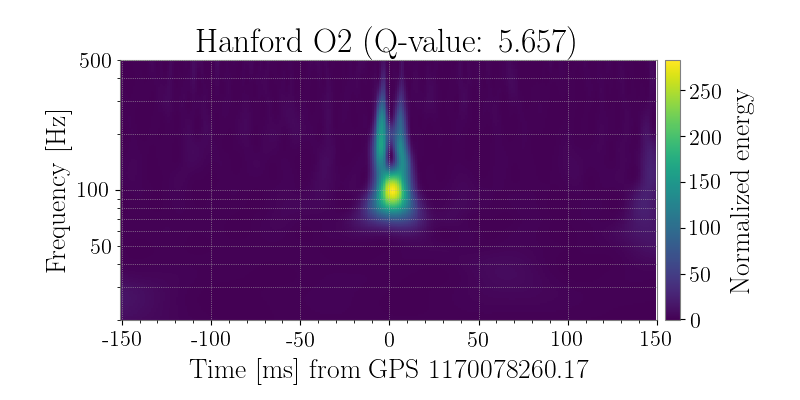
\includegraphics[width=1\linewidth]{snitch_O2}
		\caption{Snitch blip}
		\label{fig:snitch_O2}
	\end{subfigure}
	\caption{Six possible subclasses of blips.}
	\label{fig:six}
\end{figure}

The variance in the background of each image is due to the relative energy of each blip. In this figure, the dot blip (figure \ref{fig:dot_O2}) has a relatively low energy compared to the normal blip (figure \ref{fig:normal_O2}), which is why the normal blip is so clear. However, I also found high energy dots and low energy normals in my image database. The double-blip, on the other hand, appears to always have relatively low energy, and it always has one low-frequency dot shape around 100 ms away from the mid-frequency, lower duration signal that causes the omicron trigger. It is unclear whether this is simply a coincidence, where two blips just so happen to be practically on top of each other, or if these are two connected signals in a cause-effect relationship, or if the low-frequency dot is simply a side effect of the whitening of the Q-transform.

The hat blip, similar to the double-blip, is a complete mystery. The name comes from the wavy, squiggly nature of its shape, which is very different from the symmetry present in all the other types of blips (other than double-blips). The base of the hat in figure \ref{fig:hat_O2} is at a fairly low frequency, but the bases of other hats are a slightly higher frequency, and all hats follow the general shape of a wavy top and a more spread-out, wavy bottom. One consistency among hat blips is their general frequency range, which is low- to mid-frequency.

The last new blip is the snitch, which has two vertical, upward trails on either side of a round ball. Similar to other blip types, the snitch occurs at both high and low frequency. 

\section{Determining Distinguishable Characteristics of Possible Sub-Classifications of Blip Glitches} \label{plots}

Now that I had a fairly robust idea of the possible subclassifications of blips, I searched for characteristics that could distinguish one type from another. The first step I took in finding specific attributes to sub-classify the blip glitches was to create a variety of histograms examining possible characteristics to find clusters of blips that might correspond to the six different types. I started with peak frequency and found a striking difference between the Livingston blips and the Hanford blips, as shown in figure \ref{fig:combined} on page \pageref{fig:combined_peakf}. Since the scale is dependent on the Hanford blips, figure \ref{fig:llo_peakf} shows the Livingston blips by themselves.

\begin{figure}[h!]
	\centering
	\begin{subfigure}{.49\textwidth}
		\centering
		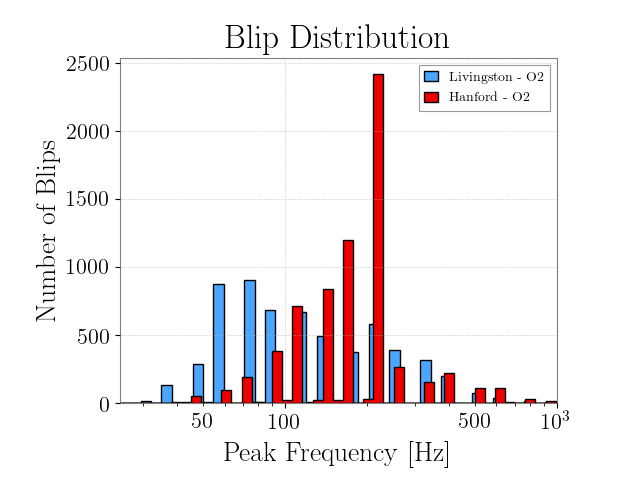
\includegraphics[width=1\linewidth]{combined_peakf}
		\caption{All O2 blips from Hanford and Livingston.}
		\label{fig:combined}
	\end{subfigure}
	\begin{subfigure}{.49\textwidth}
		\centering
		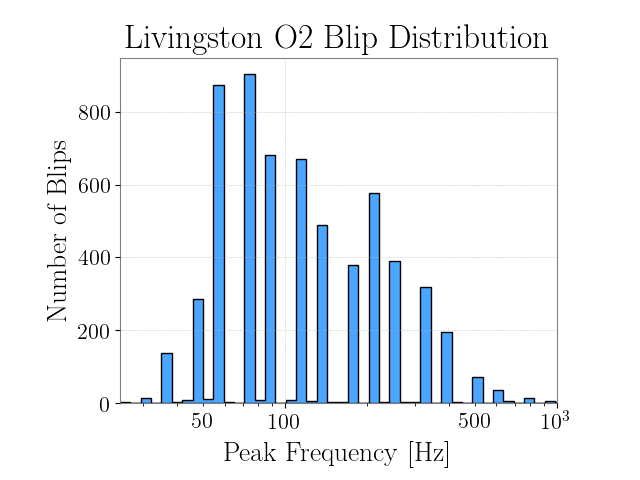
\includegraphics[width=1\linewidth]{llo_peakf}
		\caption{Livingston blips}
		\label{fig:llo_peakf}
	\end{subfigure}
	\caption{}
	\label{fig:combined_peakf}
\end{figure}

These histograms show a clear difference between the Livingston blips and the Hanford blips, which is somewhat surprising considering that all six blip shapes are found in both detectors. Most of the Hanford blips appear to have a peak frequency of 200 Hz, with a fairly steep dropoff on both sides of the 200 Hz spike. The Livingston blips, on the other hand, look to be more evenly spread out among the different frequencies, and there are considerably more low-frequency blips at Livingston. One possible explanation for this is that Livingston just happens to be more sensitive at low frequencies. 

To get a closer look at the Livingston blips and see if there is anything significant going on within Hanford's 200 Hz spike, I made 2D histograms plotting peak frequency versus SNR (signal to noise ratio) for each detector. Figure \ref{fig:hists_2d}  on page \pageref{fig:hists_2d} shows these histograms. Here, the differences between Livingston and Hanford are even more clear. For example, while Livingston's peak frequency distribution (figure \ref{fig:llo_peakf}) does show a local maxima around 200 Hz, the 2D histogram of Livingston reveals that most of those blips have a low SNR, whereas a considerable amount of Hanford 200 Hz blips have a high SNR. 

\begin{figure}[h!]
	\centering
	\begin{subfigure}{.49\textwidth}
		\centering
		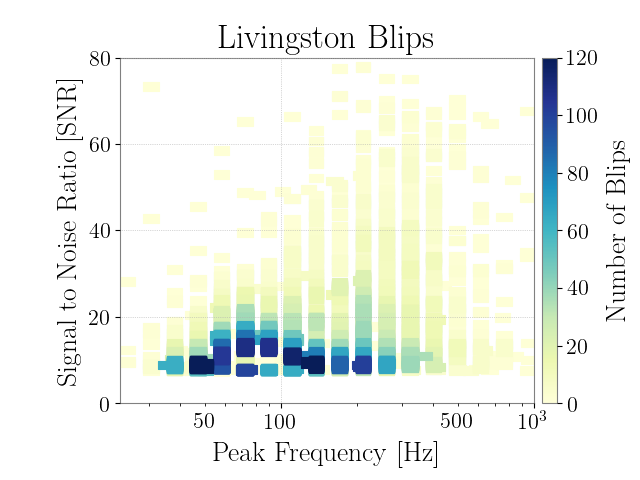
\includegraphics[width=1\linewidth]{llo_2d}
		%\caption{Livingston 2D histogram}
		\label{fig:llo_2d}
	\end{subfigure}
	\begin{subfigure}{.49\textwidth}
		\centering
		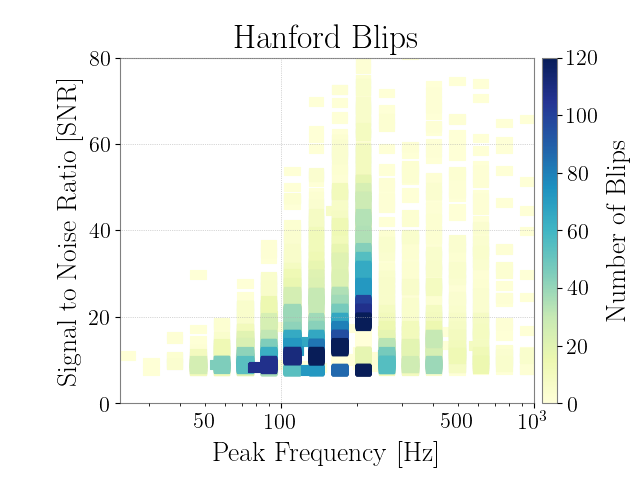
\includegraphics[width=1\linewidth]{lho_2d}
		%\caption{Hanford 2D histogram}
		\label{fig:lho_2d}
	\end{subfigure}
	\caption{2D histograms of the O2 blips from Livingston and Hanford.}
	\label{fig:hists_2d}
\end{figure}

Looking at the broader shape of each 2D histogram, both appear to have a clear arc shape over a range of frequencies, where an increase in frequency also increases the SNR, and then at even higher frequencies, the SNR decreases. At Livingston, it starts with low-SNR blips around 50 Hz and ends around 150 Hz. At Hanford, we can see the same general arc from about 80 Hz to the low-SNR blips at 200 Hz, but the high-SNR blips at 200 Hz are clearly separate from the arc. The similarity in the arcs from both detectors raise interesting hypotheses. For example, the blips at the start of each arc might be similar, even though the peak frequencies are different. 

One data point that hasn't been mentioned so far is central frequency. Although it is similar to peak frequency, it might shed more light on the similarities between the Hanford and Livingston blips and the 200 Hz blips at Hanford. I created another two 2D histograms, one each for Hanford and Livingston, this time plotting central frequency versus peak frequency. The histograms are in figure \ref{fig:central_hists}.

\begin{figure}[h!]
	\centering
	\begin{subfigure}{.49\textwidth}
		\centering
		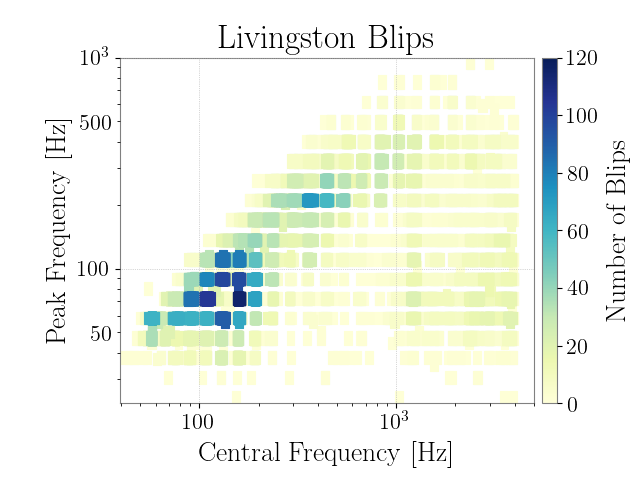
\includegraphics[width=1\linewidth]{llo_peak_v_centr}
		%\caption{Livingston 2D histogram}
		\label{fig:llo_centr}
	\end{subfigure}
	\begin{subfigure}{.49\textwidth}
		\centering
		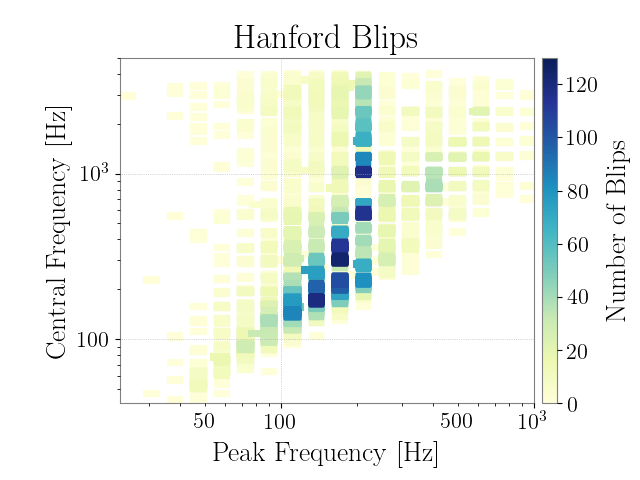
\includegraphics[width=1\linewidth]{lho_peak_v_centr}
		%\caption{Hanford 2D histogram}
		\label{fig:lho_centr}
	\end{subfigure}
	\caption{Central frequency versus peak frequency 2D histograms of blips from O2.}
	\label{fig:central_hists}
\end{figure}

Now, any similarities between the two detectors start to dissolve. The high-density bins at Livingston create a completely different overall shape than those at Hanford. One thing that is especially interesting is the 200 Hz peak at Livingston, which has the highest-density bin around 350 Hz central frequency, and at Hanford, 350 Hz is one of the few places along the 200 Hz peak frequency bin where there are hardly any blips. Additionally, the histogram of Hanford reveals at least three different clusters of blips within the 200 Hz peak, which could distinguish some of those blips from each other. 

All the 2D histograms have high density bins, and we can use neural networks to investigate these possible clusters and see if any of them correspond to the six types of blips I identified in section \ref{O2}. 

\section{Neural Network Implementation}

At this point in the project, Neural Networks become more desirable than histograms and manual searching. We want to know if the six types of blips can be identified by a computer, not just one person looking at a couple hundred images. If a Neural Network can be used to find the differences between the types of blips, then we know that sub-classification is possible and can be implemented in GravitySpy to classify all blips and find their sources.

\subsection{Building a Neural Network}

There are countless ways to build and implement a Neural Network. The first step is deciding what type of learning we want: supervised learning, reinforcement learning, or unsupervised learning. Reinforcement learning can almost immediately be discarded. Since it depends on a function to reward the program, it is not very helpful for image classification, which cannot be easily translated into better states versus worse states. The ideal technique is unsupervised learning because we have a guess as to the number of classes and we don't have a large dataset of images that are already classified into those classes. However, unsupervised learning is extremely complex and only effective when there are clear subclasses to be found. Supervised learning, on the other hand, is a more accurate method because the neural network is trying to classify already-labeled data and therefore has a much better gauge of accuracy. Unfortunately, since we are trying to identify the classes themselves, this learning technique is also not ideal for our purposes, especially because I only have about 250 sub-classified blips that can serve as a labeled dataset. As a result, I implemented both supervised and unsupervised learning neural networks.

The next step in creating a neural network is deciding the type of layers to put in the network. Since I want my input set to consist of images, I used Convolutional Neural Networks (CNNs) in both the supervised and unsupervised models. CNNs are better for images than a normal dense layer because they take all the surrounding points into consideration. Each image is stored as a multi-dimensional array, but normal dense layers can only interpret a single array, and can therefore only take into account pixels that are horizontally next to each other. CNNs, on the other hand, take in multi-dimensional arrays as input and use all the surrounding pixels to learn about the image. 

The last thing to do before creating the neural networks themselves is to create the input dataset, i.e. the images. I created a database of all the blips from Hanford and Livingston during O2, by plotting Q-transforms with a standardized time domain (20 seconds), cropped down to 0.22 seconds, similar to the previous images I created. I left the energy (colorbar) to scale itself during the calculation, mostly because the disparity between blips with low energy and blips with high energy is so drastic that the shapes become difficult to distinguish with a standardized energy scale. An example of the images in the database is in figure \ref{fig:image}. Since there are no axes or titles, the images are labeled with their GPS time and detector from their file names. This also allows access to the images of specific blips during future searches, which is helpful for supervised learning.

\begin{figure}[h!]
	\centering
	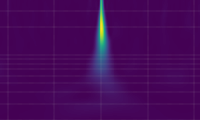
\includegraphics[width=.4\linewidth]{image}
	\caption{An example of the 120 x 200 images in the database used as input into neural networks.}
	\label{fig:image}
\end{figure}

\subsection{Supervised Learning Neural Network}

The goal of a supervised learning neural network is to see whether specific attributes of blips create clusters. We can label specific blips based on their omicron trigger values, and then evaluate the correlation based on the accuracy of the trained neural network. For example, I can label all the 200 Hz blips from Livingston with a "1," and label all the 200 Hz blips from Hanford with a "0," and see if the neural network can distinguish one "class" from another. If the Hanford 200 Hz blips are fundamentally different than the ones at Livingston (which would be assumed, based on the histogram plots in section \ref{plots}), the neural network should have a high accuracy and "classify" the blips easily.

The example above is a case of binary classification, but we can create a neural network with as many classes as we want. Additionally, most neural networks have one input, but we can also create a two-input neural network that takes in both images and auxiliary data from the omicron trigger. As a result, I created four neural networks templates: one-input binary, two-input binary, one-input multi-class, and two-input multi-class. All four have almost exactly the same network of layers, but since they all have different uses, it is easy to implement different ideas. A condensed version of the layers in both of the two-input neural networks is in figure \ref{fig:sup_condensed}. The only difference between the two-input CNN and the one-input CNN is that the \texttt{Flatten()} layer goes straight to the first \texttt{Dense()} layer with only one input. To make this network multi-class instead of binary, the output shape of the \texttt{main\_output} layer is changed from 1 to the number of classes, and the loss function is changed from \texttt{binary\_crossentropy} to \texttt{categorical\_crossentropy}.

\begin{figure}[h!]
	\centering
	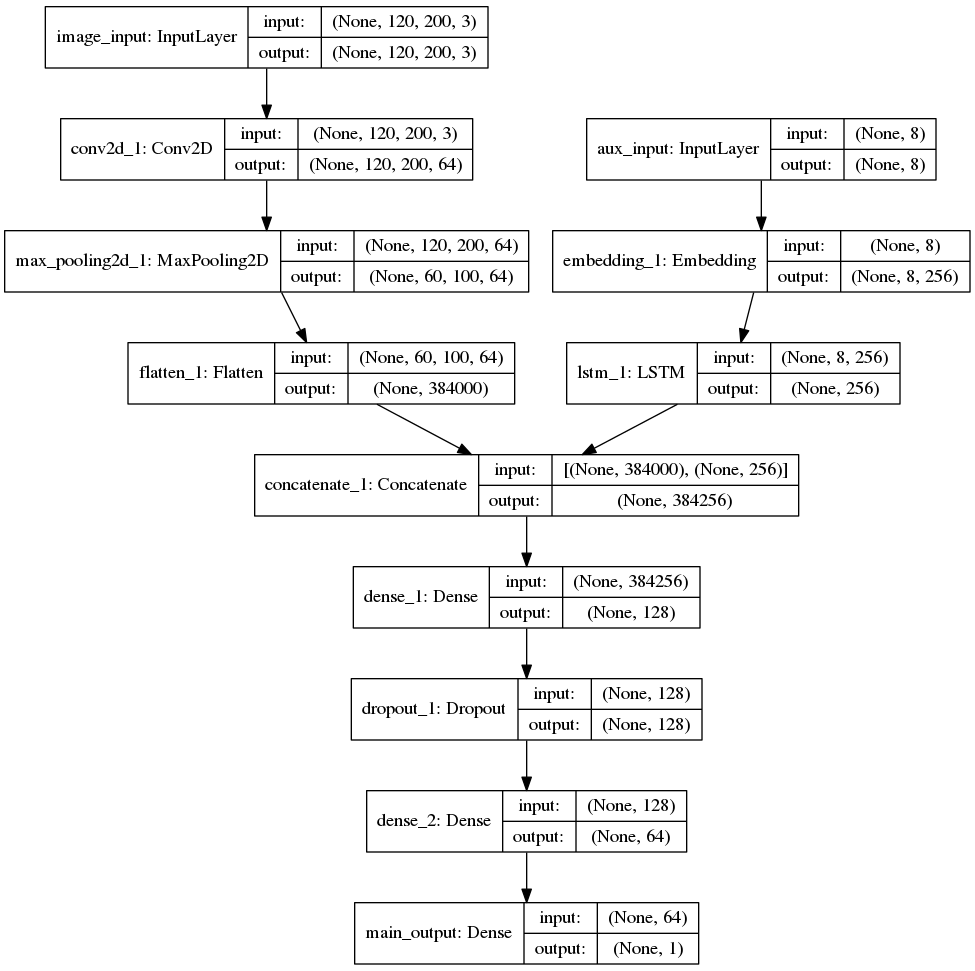
\includegraphics[width=.5\linewidth]{sup_condensed}
	\caption{Condensed version of my two-input Convolutional NN. There are additional \texttt{Conv2D()} and \texttt{MaxPooling2D()} layers between the \texttt{Input()} layer and the \texttt{Flatten()} layer, and an additional \texttt{Dropout()} and \texttt{Dense()} layer before the \texttt{main\_output}.}
	\label{fig:sup_condensed}
\end{figure}

The auxiliary input consists of about 6-12 omicron data values, including but not limited to q-value, confidence, SNR, bandwidth, duration, interferometer, and image status. The shape of the auxiliary input varies depending on what "classes" the neural network is looking at. Going back to the earlier example about distinguishing Livingston 200 Hz blips from Hanford 200 Hz blips, that auxiliary input would not include the interferometer or the peak frequency of each blip. 

Although adding auxiliary input seems helpful because it gives the neural networks more information, the performance difference between one-input neural networks and two-input neural networks is practically non-existent. Using images by themselves is exactly the same as using images along with auxiliary data. This is consistent with GravitySpy, which is directly dependent on images. The auxiliary data is not robust enough to aid in classification, both in GravitySpy's glitch classification and this project's sub-classification of blips. As a result, I mostly use the one-input neural networks. A summary of the different supervised learning neural networks that I ran and their conclusions and implications is in the next section.

\subsubsection{Results of Supervised Network}

As mentioned in the previous section, I first started with both one-input and two-input neural networks. Results in table \ref{table:1}.

%black, blue, brown, cyan, darkgray, gray, green, lightgray, lime, magenta, olive, orange, pink, purple, red, teal, violet, white, yellow

\begin{table}[h!]
\centering
\begin{tabular}{||c c c c c c||} 
 \hline
 NN & Input & Classes & (Training, Testing) & End Loss & Test Accuracy \\ [0.5ex] 
 \hline\hline
 \multirow{2}{*}{\hfil 1} & One-input & Binary & (573,63) & 0.5310 & 0.8571 \\ 
  & Two-input & Binary & (573,63) & 0.5288 & 0.8571 \\ 
  \multirow{2}{*}{\hfil 2} & One-input & Binary & (1178,130) & 0.6792 & 0.3540 \\ 
  & Two-input & Binary & (1178,130) & 0.6824 & 0.3540 \\
 \rowcolor{pink}
  & One-input & Binary & (521,57) & 0.6643 & 0.0702 \\
  \rowcolor{pink}
 \multirow{-2}{*}{\hfil 3}& Two-input & Binary & (521,57) & 0.6640 & 0.0877 \\
 4 & One-input & Binary & (1196,132) & 0.6956 & 0.1288 \\
 5 & One-input & Binary & (1717,190) & 0.6099 & 0.3271 \\
 6 & One-input & Binary & (369,41) & 0.6255 & 0.7317 \\
 7 & One-input & Binary & (509,56) & 0.6215 & 0.6786 \\
 8 & One-input & Binary & (455,50) & 0.6831 & 0.5601 \\
 9 & One-input & Binary & (938,104) & 0.6935 & 0.4808 \\
 \rowcolor{pink}
 10 & One-input & Multi & (1089,181) & 1.4652 & 0.3923 \\
 \hline
\end{tabular}
\caption{Table to test captions and labels}
\label{table:1}
\end{table}

\subsection{Unsupervised Neural Network}

For my unsupervised neural network, I modified public source code\footnote{\href{https://github.com/keras-team/keras/blob/master/examples/variational_autoencoder.py}{GitHub source code}} to make a Variational Autoencoder (VAE). This type of unsupervised neural network consists of an encoder and a decoder, where Bayesian statistic techniques are used between the encoder and decoder to better predict what the data should look like. Unlike supervised learning, which outputs a value corresponding to a class, autoencoders output new images. The neural network trains itself by trying to create as close to the same image as what was put in. Once the neural network is trained, the test images then get put through the encoder part of the neural network, which also outputs meaningful statistical values. We can then create a scatter plot of the statistical values from the test images and see if there are visible clusters \cite{Kingma:2013}. 

Since VAEs are so complex, it is difficult to implement convolutional layers within the autoencoder, especially when the input data is so large. However, I managed to sneak in a few layers into the encoder without overloading memory. The layers of the VAE neural network are in figure \ref{fig:vae}.

\begin{figure}[h!]
	\centering
	\begin{subfigure}{.49\textwidth}
		\centering
		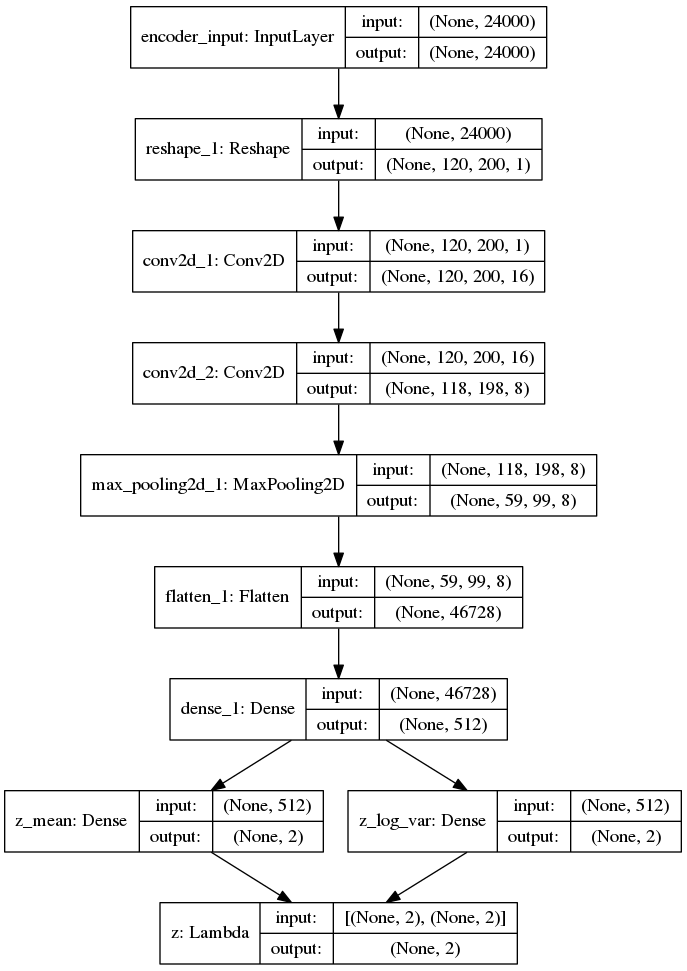
\includegraphics[width=1\linewidth]{vae_mlp_encoder}
		\caption{Convolutional encoder layers}
		\label{fig:encoder}
	\end{subfigure}
	\begin{subfigure}{.49\textwidth}
		\centering
		\begin{subfigure}{.6\textwidth}
			\centering
			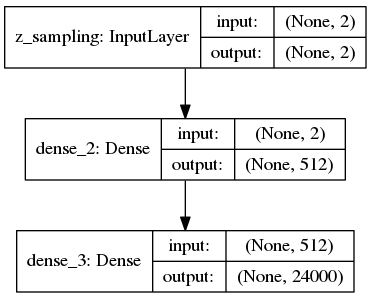
\includegraphics[width=1\linewidth]{vae_mlp_decoder}
			\caption{Decoder layers}
			\label{fig:vae_decoder}
		\end{subfigure}
		\vspace{10mm}%
		\begin{subfigure}{.8\textwidth}
			\centering
			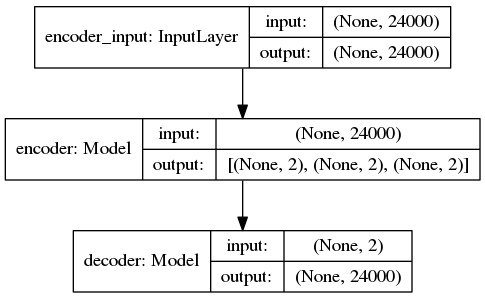
\includegraphics[width=1\linewidth]{vae_mlp}
			\caption{Combined model summary}
			\label{fig:vae_mlp}
		\end{subfigure}
		%\caption{Decoder layers}
		\label{fig:decoder}
	\end{subfigure}
	
	\caption{Layers of a Variational Autoencoder.}
	\label{fig:vae}
\end{figure} 

The output of interest from the VAE is the statistical plot that can reveal clusters of data. The VAE can be run both without any assumed classes and with labels that we think correspond to clusters. Finding clusters is especially important for future sub-classification because the success of sub-classification could depend on how easily the blips cluster during unsupervised learning. If no clusters are found, it is likely to be extremely difficult for a neural network to distinguish between the different types of blips, no matter how easy it is for us to see the differences by eye. The next section goes through the clustering found by my VAE.

\subsubsection{Results of Unsupervised Network}

The first 


\bibliography{references}
\bibliographystyle{ieeetr}

\end{document}












